\documentclass[12pt,ngerman]{beamer}

\usepackage[utf8]{inputenc}
\usepackage[T1]{fontenc}
\usepackage{booktabs}
\usepackage{babel}
\usepackage{graphicx}
\usepackage{csquotes}
\usepackage{xcolor}
\usepackage{listings}
\usepackage{mdframed}
\usepackage{tikz}

\definecolor{hellgelb}{rgb}{1,1,0.8}
\definecolor{lightgelb}{rgb}{1,1,0.8}
\definecolor{colKeys}{rgb}{0,0,1}
\definecolor{colIdentifier}{rgb}{0,0,0}
\definecolor{colComments}{rgb}{1,0,0}
\definecolor{colString}{rgb}{0,0.5,0}

\newcounter{Aufgabe}
\setcounter{Aufgabe}{1}

\usepackage{mdframed}

\newmdenv [linecolor=blue, leftmargin=0.1\textwidth,rightmargin=0.1\textwidth]{infobox}

% Venn Diagrams
% Definition of circles
\def\firstcircle{(0,0) circle (2cm)}
\def\secondcircle{(0:3cm) circle (2cm)}

\colorlet{circle edge}{blue!50}
\colorlet{circle area}{blue!20}

\tikzset{filled/.style={fill=circle area, draw=circle edge, thick},
    outline/.style={draw=circle edge, thick}}

%%% end venn

\newcommand{\Aufgabe}{%
\stepcounter{Aufgabe}%
\theAufgabe%
}

\usepackage{textcomp}
\lstset{%
	language=Python,%	
    float=hbp,%
    basicstyle=\ttfamily\footnotesize, %
    identifierstyle=\color{colIdentifier}, %
    keywordstyle=\color{colKeys}, %
    stringstyle=\color{colString}, %
    commentstyle=\color{colComments}, %
    alsoletter={\_},
	language= {Python},%
    columns=flexible, %
    tabsize=2, %
    morekeywords={read_csv,system,start,close,read,isoformat,now,to_datetime,merge,to_excel,join,concat,pairplot,vq,kmeans,savefig,Series,axis,DataFrame,index,to_frame,loc,iloc,idx,mean,describe,std,count,},%
    frame=single, %
    extendedchars=true, %
    showspaces=false, %
    showstringspaces=false, %
    numbers=left, %
    numberstyle=\tiny, %
    upquote=true,
    breaklines=true, %
    backgroundcolor=\color{yellow!15}, %
    breakautoindent=true, %
    captionpos=b%
}


\lstset{literate=%
    {Ö}{{\"O}}1
    {Ä}{{\"A}}1
    {Ü}{{\"U}}1
    {ß}{{\ss}}1
    {ü}{{\"u}}1
    {ä}{{\"a}}1
    {ö}{{\"o}}1
    {~}{{\textasciitilde}}1
}

\newcommand{\pyc}[1]{\lstinline[language={Python}]{#1}}


\author{Dr. Uwe Ziegenhagen}
\title{Python \& \LaTeX}
\subtitle{Dante e.\,V. Frühjahrstagung 2017}
\date{22. März 2017}

\begin{document}

\begin{frame}

{\large Diejenigen, die aktiv mitmachen wollen, setzen sich bitte nach vorn.}

\end{frame}

\begin{frame}

\maketitle

\end{frame}


\begin{frame}
\frametitle{Überblick}
\framesubtitle{Was machen wir heute?}

\begin{itemize}
\item Python Grundlagen
\item Python in \LaTeX\ Dokumenten
\item Erzeugung von \LaTeX\ Dokumenten
\end{itemize}
\end{frame}


\begin{frame}
\frametitle{Voraussetzungen}
\framesubtitle{Was wird benötigt}

\begin{itemize}
\item Aktuelle \TeX\ Installation
\item Python3 Installation, vorzugsweise Anaconda/Winpython
\item Pakete:
\begin{itemize}
	\item numpy
	\item jinja2
	\item pandas
\end{itemize}
\item Diese Folien und Code-Beispiele unter: 
\end{itemize}

\url{https://github.com/UweZiegenhagen/PythonAndLaTeX}

\end{frame}


\begin{frame}
\frametitle{\enquote{Scientific Python} Distributionen}
\framesubtitle{~}

\begin{itemize}
	\item Linux/MacOS X kommen mit Python, aber nicht SciPy
	\item Manuell nachinstallieren oder \enquote{echte} Installation
	\item Meine Empfehlung: Anaconda
\begin{itemize}
	\item Anaconda (\url{https://www.continuum.io/downloads})
	\item WinPython (\url{https://winpython.github.io})
\end{itemize}
	\end{itemize}
	
\begin{center} % left bottom right top
\fbox{\includegraphics[width=\textwidth]{Bilder/anaconda}}
\end{center}	
\end{frame}

\begin{frame}
\frametitle{Das SciPy Framework}
\framesubtitle{~}

Neben \texttt{pandas} ist enthalten:

\begin{description}
\item[NumPy] matrices, vectors, algorithms
\item[IPython] Matlab/Mathematica-like environment 
\item[Matplotlib] scientific plotting, basis for \texttt{seaborn} library
\item[SymPy] symbolic mathematics
\item [\ldots] etc, etc.
\end{description}
\end{frame}


\begin{frame}[containsverbatim]
\frametitle{Testen der Installation}

\begin{itemize}
	\item Funktionieren die folgenden Befehle?
\end{itemize}

\begin{lstlisting}
import jinja2
import pandas
import numpy
\end{lstlisting}
\end{frame}

\section{Python Grundlagen}

\begin{frame}
\frametitle{Python}
\framesubtitle{~}

\begin{itemize}
	\item Erfunden von Guido van Rossum (Niederlande)
	\item Fokus auf lesbaren und verständlichen Code
	\item \enquote{batteries included} $\Rightarrow$ umfangreiche Standardbibliothek
	\item Mein erster Kontakt mit Python: Downloadskript für den SaveTV Online-VCR
	\item Python2 versus Python3 $\Rightarrow$ Python3
	\item Editor? Ich nutze Spyder3, auch empfehlenswert: Geany
	\item Python selbst liefert IDLE mit
\end{itemize}
\end{frame}

\begin{frame}[fragile]
\frametitle{Python \enquote{Hello World}}

\lstinputlisting[firstline=7,caption={Hello World in Python 3.x, sources/helloWorld.py}]{sources/helloWorld.py}

\end{frame}


\begin{frame}[fragile]
\frametitle{Strings, Listen und Tupel}
\framesubtitle{Strings}

\lstinputlisting[firstline=7,caption={Strings, sources/Strings.py}]{sources/Strings.py}

\end{frame}

\begin{frame}[fragile]
\frametitle{Strings, Listen und Tupel}
\framesubtitle{Stringfunktionen}

\lstinputlisting[firstline=7,caption={Strings, sources/Strings2.py}]{sources/Strings2.py}
\end{frame}


\begin{frame}[fragile]
\frametitle{Strings, Listen und Tupel}
\framesubtitle{Listen}

\begin{itemize}
	\item Index von $0$ bis $n-1$
	\item veränderbar
\end{itemize}

\lstinputlisting[firstline=8,caption={Listen, sources/Listen.py}]{sources/Listen.py}

\end{frame}


\begin{frame}[fragile]
\frametitle{Strings, Listen und Tupel}
\framesubtitle{Tupel}

\begin{itemize}
	\item ähnlich wie Listen
	\item Index von $0$ bis $n-1$
	\item nicht veränderbar, also \enquote{schreibgeschützt}
\end{itemize}


\lstinputlisting[firstline=7,caption={Tupel, sources/Tupel.py}]{sources/Tupel.py}
\end{frame}


\begin{frame}[fragile]
\frametitle{Dictionaries}
\framesubtitle{Key-Value Paare}

\begin{itemize}
	\item nicht veränderbar
\end{itemize}


\lstinputlisting[firstline=7,caption={Tupel, sources/Dictionaries.py}]{sources/Dictionaries.py}
\end{frame}

\section{Programmfluss}

\begin{frame}[fragile]
\frametitle{Flusssteuerung}
\framesubtitle{if/then}

\lstinputlisting[firstline=7,caption={if-then, sources/ifthen.py}]{sources/ifthen.py}

"condition"\ kann ein üblicher Boolean Ausdruck sein.

\end{frame}

\begin{frame}[fragile]
\frametitle{Flusssteuerung}
\framesubtitle{for}

\lstinputlisting[firstline=7,caption={for-Schleifen, sources/for.py}]{sources/for.py}

\end{frame}

\begin{frame}[fragile]
\frametitle{Flusssteuerung}
\framesubtitle{while}

\lstinputlisting[firstline=7,caption={while-Schleifen, sources/while.py}]{sources/while.py}

\end{frame}

\begin{frame}[fragile]
\frametitle{Funktionen}
\framesubtitle{~}

\lstinputlisting[firstline=7,caption={Definition von Funktionen, sources/Funktionen.py}]{sources/Funktionen.py}

\end{frame}


\begin{frame}[fragile]
\frametitle{Ein- und Ausgabe}
\framesubtitle{Kommandozeile}

\lstinputlisting[firstline=7,caption={Ein- und Ausgabe: Kommandozeile, sources/io.py}]{sources/io.py}

\end{frame}

\begin{frame}[fragile]
\frametitle{Ein- und Ausgabe}
\framesubtitle{Dateien lesen}

\lstinputlisting[firstline=7,caption={Ein- und Ausgabe: Dateien,sources/readWriteFile.py}]{sources/readWriteFile.py} 

\begin{itemize}
	\item Um Excel, CSV und ähnliches zu lesen $\Rightarrow$ pandas sehr empfehlenswert
\end{itemize}
\end{frame}


\begin{frame}[fragile]
\frametitle{Ein- und Ausgabe}
\framesubtitle{UTF8-Dateien lesen und schreiben}

\lstinputlisting[firstline=7,caption={UTF8, sources/readWriteUTF8.py}]{sources/readWriteUTF8.py} 

\end{frame}

\begin{frame}[fragile]
\frametitle{Andere wichtige Befehle}
\framesubtitle{Das \texttt{os} Modul}

\begin{itemize}
\item \lstinline{os.system(<Befehl>)} Führt externen Befehl aus
\item \lstinline{os.start(<Datei>)} Öffnet Datei mit der Standard-Applikation (nur unter Windows)
\end{itemize}
\end{frame}

\begin{frame}[fragile]
\frametitle{Aufgabe \theAufgabe}
\framesubtitle{~}

\begin{itemize}
\item Wir erzeugen Rechenaufgaben für Kinder
\item links die Aufgabe, rechts die Lösung
\item Aufgaben randomisiert (\texttt{random} Modul)
\item Datei automatisch übersetzen und ausführen
\item Tipp für Font: TeX Gyre Schola, \verb|\usepackage{tgschola}|
\end{itemize}
\end{frame}

\section{Python in \LaTeX-Dokumenten}

\begin{frame}
\frametitle{Python und \LaTeX\ verbinden}
\framesubtitle{~}

Q: Wie kann man \LaTeX~ und Python in nur einem Dokument verwalten?

A: Literate programming\footnote{WEB, CWEB, NOWEB, SWEAVE, knitR}

\begin{itemize}
\item etwas \enquote{Selbstgestricktes}
\item Python\TeX\ von Ge­of­frey M. Poore \url{https://www.ctan.org/pkg/pythontex}
\end{itemize}
\end{frame}

\begin{frame}[fragile]
\frametitle{Python im \LaTeX-Lauf}

\begin{lstlisting}[basicstyle={\ttfamily\footnotesize},language={TeX},morekeywords={makeatletter,endVerbatimOut,typeout,lstinputlisting,makeatother,VerbatimOut,footnotesize}]
\makeatletter
\newenvironment{pycode}[1]%
  {\xdef\d@tn@me{#1}\xdef\r@ncmd{python #1.py > #1.plog}%
  \typeout{Writing file #1}\VerbatimOut{#1.py}% 
  }
  {\endVerbatimOut %
 \toks0{\immediate\write18}%
 \expandafter\toks\expandafter1\expandafter{\r@ncmd}%
 \edef\d@r@ncmd{\the\toks0{\the\toks1}}\d@r@ncmd %
 \lstinputlisting[language={Python},label=listing:\d@tn@me,basicstyle={\ttfamily\footnotesize}]{\d@tn@me.py}%
 \lstinputlisting[basicstyle={\ttfamily\footnotesize}]{\d@tn@me.plog}%
}
\makeatother
\end{lstlisting}

\begin{itemize}
	\item Beispiele unter \texttt{/sources}, leicht anpassbar
\end{itemize}

\end{frame}

\begin{frame}
\frametitle{Python\TeX}

\begin{itemize}
\item \enquote{PythonTeX} Paket von Ge­of­frey M. Poore
\item Paket in Version 0.15 auf CTAN, in \TeX~Live enthalten
\item unter Windows \texttt{pythontex.exe}
\item stellt mehrere Befehle und Umgebungen bereit
\end{itemize}
\end{frame}

\begin{frame}[fragile]
\frametitle{Python\TeX}

Befehle

\begin{itemize}
\item \verb|\py{}|  für Code, der einen String zurückliefert
\item \verb|\pyc{}|  für Code, der nur ausgeführt wird
\item \verb|\pys{}|  mit Substitution
\item \verb|\pyv{}|  für Code, der nur gesetzt wird
\item \verb|\pyb{}|  für Ausführung und Satz der Ergebnisse
\end{itemize}

Umgebungen

\begin{description}
\item[pycode] wie \texttt{pyc}
\item[pysub] wie \texttt{pys}
\item[pyverbatim] wie \texttt{pyv}
\item[pyblock] wie \texttt{pyb}
\item[pyconsole] simuliert eine Python-Konsole
\end{description}

\end{frame}

\begin{frame}
\frametitle{Python\TeX}
\framesubtitle{Arbeitsweise}



\end{frame}

\begin{frame}[fragile]
\frametitle{Arara-Regel}

\begin{itemize}
	\item Was ist Arara?
	\item \url{texwelt.de/wissen/fragen/8764/was-ist-arara}
\end{itemize}

\lstinputlisting[caption={UTF8, sources/pythontex.yaml},basicstyle=\ttfamily\scriptsize]{sources/pythontex.yaml} 


\end{frame}

\begin{frame}
\frametitle{Daten verarbeiten}
\framesubtitle{Die wunderbare Welt von \texttt{pandas}}

\begin{itemize}
\item mein \enquote{täglich Brot}: Datenbestände zwischen Banksystemen abgleichen 
\item \enquote{pandas is an open source, BSD-licensed library providing high-performance, easy-to-use data structures and data analysis tools for the Python programming language.}\footnote{Source: \url{pandas.pydata.org}}
\item Initiiert 2008 durch Wes McKinney von AQR Capital Management für hoch-performante quantitative Analyse
\item Wesentliche Teile in C/Cython implementiert
\item  Current version is 0.19
\end{itemize}
\end{frame}

\section{Data Handling with \texttt{pandas}}

\begin{frame}
\frametitle{Series und DataFrames}

\begin{itemize}
	\item central data structures in \texttt{pandas}
\end{itemize}\vspace*{1em}

\begin{figure}
\begin{center}
\includegraphics[trim=50mm 55mm 45mm 55mm,width=0.8\textwidth]{Bilder/SeriesFrames.pdf}
\end{center}
\end{figure}
\end{frame}


\begin{frame}
\frametitle{Daten lesen}
\framesubtitle{~}

\begin{center}
\begin{tabular}{ll} \toprule
Command & Description \\ \midrule
read\textunderscore pickle &read Pickle objects \\
read\textunderscore table & for general table-like formats  \\
read\textunderscore csv & Comma-Separated Values  \\
read\textunderscore fwf & for weird fixed-width formats  \\
read\textunderscore clipboard & read from clipboard  \\
read\textunderscore excel & read Excel files \\ \bottomrule
\end{tabular}\vspace*{-0.35em}
\end{center}

other commands for HTML, JSON, HDF5, \ldots
\end{frame}

\begin{frame}[fragile]
\frametitle{Reading CSV}
\framesubtitle{~}

\begin{itemize}
\item CSV can be pretty \enquote{messed up}:
\begin{itemize}
	\item column separator
	\item decimal separator
	\item text encoding
\end{itemize}
\item see the specification: \url{http://pandas.pydata.org/pandas-docs/stable/generated/pandas.read_csv.html}
\begin{description}
\item[sep] specify the column separator
\item[thousands] Thousands separator
\item[encoding] hopefully UTF-8 (BOM!)
\item [decimal] decimal separator
\item [converters] converters=\{'A': str\} for explicit conversion
\end{description}
\end{itemize}
\end{frame}

\begin{frame}
\frametitle{Reading Excel}

\begin{itemize}
\item Use \pyc{pd.read_excel()} to read XLSX files (which are just zipped XMLs)
\item see the documentation: \url{http://pandas.pydata.org/pandas-docs/stable/generated/pandas.read_excel.html}
\item to export to Excel use \pyc{pd.to_excel()} function
\item remarks:
\begin{itemize}
	\item Excel export is much slower than CSV
	\item Exporting \enquote{styled} Excel requires additional effort
	\item Excel can be well controlled via COM (Common Object Model) 
\end{itemize}
\end{itemize}
\end{frame}

\begin{frame}[fragile]
\frametitle{Querying DataFrames}
\framesubtitle{Getting basic information}

\begin{itemize}
	\item For the next slides load \texttt{Northwind} data
	\item First task after loading data: do some sanity checks
\end{itemize}

\begin{lstlisting}[language={Python}]
customers = pd.read_excel('Northwind.xlsx',
                          sheetname = 'Customers')

print(len(customers))     # Zeilenzahl
print(customers.head()) # die ersten 5 Zeilen
print(customers.tail())   # die letzten 5 Zeilen
print(list(customers))    # die Spaltennamen
\end{lstlisting}
\end{frame}

%\begin{frame}[fragile]
%\frametitle{Selecting Data}
%\framesubtitle{Selection of rows and columns}
%
%\begin{lstlisting}[language={Python}]
%
%\end{lstlisting}
%\end{frame}

\begin{frame}[fragile]
\frametitle{Pandas Dataframe Operations}
\framesubtitle{Selection and Filtering I}

\begin{itemize}
	\item pandas provides sophisticated methods to select, filter and transform rows and columns
\end{itemize}

\begin{itemize}
\item Select only certain columns

\pyc{df = df[['colA', 'colB']]}

\item Select only first two rows (hint: index starts at 0)

\pyc{df.iloc[:1]}

\item Select only rows where column value is greater

\pyc{df[df['colA'] > 50]}
\end{itemize}
\end{frame}

\begin{frame}[fragile]
\frametitle{Pandas Dataframe Operations}
\framesubtitle{Selection and Filtering II}

\begin{itemize}
\item Select only rows where column value is greater  \newline than 50 and smaller than 500

\pyc{df[(df['colA'] > 50) | (df['colA'] < 500)]}

\item Select only rows where column value is not

\pyc{df[~(df['colA'] == 'HelloWorld')]}

\item Select those rows, where column b is 'A' or 'B'

\pyc{df = df[ (df['b'] == 'A') | (df['b'] == 'I')]}

\item more readable alternative via \pyc{isin()}

\pyc{df = df[df['b'].isin(['A','I'])]}

\item or the opposite

\pyc{df = df[~df['b'].isin(['A','I'])]}

%\item See more here: \url{http://chrisalbon.com/python/pandas_indexing_selecting.html}

\end{itemize}
\end{frame}


%\begin{frame}[fragile]
%\frametitle{Pandas Dataframe Operations}
%\framesubtitle{Combining DataFrames with \texttt{append()} and \texttt{concat()}}
%
%\begin{itemize}
%	\item 
%	\item 
%	\item
% 	\item 
%	\item 
%	\item 
%\end{itemize}
%
%
%\end{frame}



\begin{frame}[fragile]
\frametitle{Pandas Dataframe Operations}
\framesubtitle{Merging and Joining}

\begin{itemize}
\item \texttt{merge()} provides SQL-like merging
\item very handy to combine different datasets
\item Supported are the followin join-types:
\begin{itemize}
	\item Left
	\item Right
	\item Inner
	\item Full Outer
\end{itemize}
\item \texttt{join()} is special alias for \texttt{merge()},  works on  \\ index, not columns  (the default for merge)
\end{itemize}

\end{frame}

\begin{frame}[fragile]
\frametitle{Pandas Dataframe Operations}
\framesubtitle{Merging and Joining}

\begin{itemize}
	\item Default-command for \texttt{merge()}
\end{itemize}

\begin{lstlisting}
leftDataFrame.merge(rightDataFrame, how='inner', 
on=None, left_on=None, right_on=None, left_index=False, 
right_index=False, sort=False, suffixes=('_x', '_y'), 
copy=True, indicator=False)
\end{lstlisting}

\begin{enumerate}
\item define the other DataFrame to merge
\item define how to merge
\item define the keys to use for the merge
\end{enumerate}


%\begin{figure}
%\begin{center} % left bottom right top
%\fbox{\includegraphics[width=0.8\textwidth]{Bilder/merge}}
%\end{center}
%\caption{merge, source: \texttt{pandas} documentation}
%\end{figure}

\end{frame}


\begin{frame}
\frametitle{Merging}
\framesubtitle{Inner Join}

\begin{itemize}
\item Select all data which is in A and B
\end{itemize}

\begin{center}
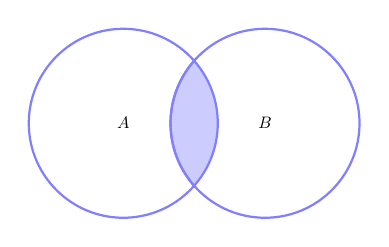
\begin{tikzpicture}[scale=0.6, every node/.style={scale=0.6}]
    \begin{scope}
        \clip \firstcircle;
        \fill[filled] \secondcircle;
    \end{scope}
    \draw[outline] \firstcircle node {$A$};
    \draw[outline] \secondcircle node {$B$};
    %\node[anchor=south] at (current bounding box.north) {$A \cap B$};
\end{tikzpicture}
\end{center}

{\footnotesize
\begin{columns}
\begin{column}{0.3\textwidth}
left \\
\begin{tabular}{c|cc} \toprule
   & A  &  Key \\ \midrule
0 & A0 &  K0 \\
1 & A1 &  K1 \\ 
2 & A2 &  K2 \\
3 & A3 &  \textcolor{red}{K4} \\ \bottomrule
\end{tabular}
\end{column}
\begin{column}{0.3\textwidth}
right \\
\begin{tabular}{c|cc} \toprule
   &  B   & Key \\ \midrule
0 &  B0 & K0 \\
1 &  B1 & K1 \\ 
2 &  B2 & K2 \\
3 &  C3 & \textcolor{red}{K5} \\ \bottomrule
\end{tabular}\end{column}
\begin{column}{0.3\textwidth}
merged \\
\begin{tabular}{c|ccc} \toprule
   & A  & B   & Key \\ \midrule
0 & A0 & B0 & K0 \\
1 & A1 & B1 & K1 \\ 
2 & A2 & B2 & K2 \\ \bottomrule
\end{tabular} \\
\vspace*{1.5em}
\end{column}
\end{columns}}


\end{frame}

\begin{frame}
\frametitle{Merging}
\framesubtitle{Left Join}

\begin{itemize}
\item Select all data which is in A and B
\end{itemize}

\begin{center}
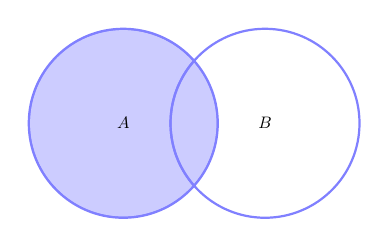
\begin{tikzpicture}[scale=0.6, every node/.style={scale=0.6}]
    \begin{scope}
        \clip \firstcircle;
        \draw[filled] \firstcircle node {$A$}
                                     \secondcircle;
    \end{scope}
    \draw[outline] \firstcircle
                   \secondcircle node {$B$};
    %\node[anchor=south] at (current bounding box.north) {$A - B$};
\end{tikzpicture}
\end{center}

{\footnotesize
\begin{columns}
\begin{column}{0.3\textwidth}
left \\
\begin{tabular}{c|cc} \toprule
   & A  &  Key \\ \midrule
0 & A0 &  K0 \\
1 & A1 &  K1 \\ 
2 & A2 &  K2 \\
3 & A3 &  \textcolor{red}{K4} \\ \bottomrule
\end{tabular}
\end{column}
\begin{column}{0.3\textwidth}
right \\
\begin{tabular}{c|cc} \toprule
   &  B   & Key \\ \midrule
0 &  B0 & K0 \\
1 &  B1 & K1 \\ 
2 &  B2 & K2 \\
3 &  C3 & \textcolor{red}{K5} \\ \bottomrule
\end{tabular}\end{column}
\begin{column}{0.3\textwidth}
merged \\
\begin{tabular}{c|ccc} \toprule
   & A  & B   & Key \\ \midrule
0 & A0 & B0 & K0 \\
1 & A1 & B1 & K1 \\ 
2 & A2 & B2 & K2 \\ \bottomrule
3 & A3 & NaN & K4 \\ \bottomrule
\end{tabular} \\
\vspace*{0.4em}
\end{column}
\end{columns}}

\end{frame}

\begin{frame}
\frametitle{Merging}
\framesubtitle{Right Join}

\begin{itemize}
\item Select all data which is in B
\end{itemize}

\begin{center}
% Right Join
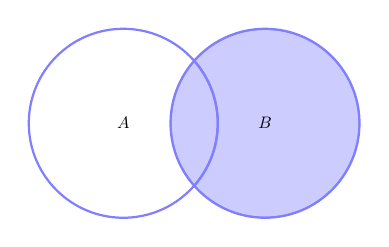
\begin{tikzpicture}[scale=0.6, every node/.style={scale=0.6}]
    \begin{scope}
        \clip \secondcircle;
        \draw[filled] \firstcircle \secondcircle node {$B$};
    \end{scope}
    \draw[outline] \firstcircle node {$A$}
                   \secondcircle;
    %\node[anchor=south] at (current bounding box.north) {$B - A$};
\end{tikzpicture}

\end{center}

{\footnotesize
\begin{columns}
\begin{column}{0.3\textwidth}
left \\
\begin{tabular}{c|cc} \toprule
   & A  &  Key \\ \midrule
0 & A0 &  K0 \\
1 & A1 &  K1 \\ 
2 & A2 &  K2 \\
3 & A3 &  \textcolor{red}{K4} \\ \bottomrule
\end{tabular}
\end{column}
\begin{column}{0.3\textwidth}
right \\
\begin{tabular}{c|cc} \toprule
   &  B   & Key \\ \midrule
0 &  B0 & K0 \\
1 &  B1 & K1 \\ 
2 &  B2 & K2 \\
3 &  C3 & \textcolor{red}{K5} \\ \bottomrule
\end{tabular}\end{column}
\begin{column}{0.3\textwidth}
merged \\
\begin{tabular}{c|ccc} \toprule
   & A  & B   & Key \\ \midrule
0 & A0 & B0 & K0 \\
1 & A1 & B1 & K1 \\ 
2 & A2 & B2 & K2 \\ 
3 & NaN & B3 & K5 \\ \bottomrule
\end{tabular} \\
\vspace*{0.4em}
\end{column}
\end{columns}}

\end{frame}


\begin{frame}
\frametitle{Merging}
\framesubtitle{Full Outer Join}

\begin{itemize}
\item Select all data which is in A or B
\end{itemize}

\begin{center}
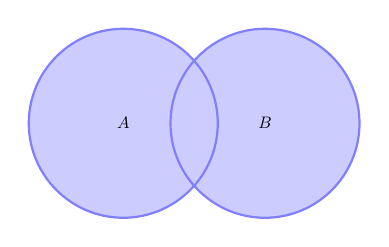
\begin{tikzpicture}[scale=0.6, every node/.style={scale=0.6}]
    \draw[filled] \firstcircle node {$A$}
                  \secondcircle node {$B$};
    %\node[anchor=south] at (current bounding box.north) {$A \cup B$};
\end{tikzpicture}
\end{center}

{\footnotesize
\begin{columns}
\begin{column}{0.3\textwidth}
left \\
\begin{tabular}{c|cc} \toprule
   & A  &  Key \\ \midrule
0 & A0 &  K0 \\
1 & A1 &  K1 \\ 
2 & A2 &  K2 \\
3 & A3 &  \textcolor{red}{K4} \\ \bottomrule
\end{tabular}
\vspace*{1.2em}
\end{column}
\begin{column}{0.27\textwidth}
right \\
\begin{tabular}{c|cc} \toprule
   &  B   & Key \\ \midrule
0 &  B0 & K0 \\
1 &  B1 & K1 \\ 
2 &  B2 & K2 \\
3 &  C3 & \textcolor{red}{K5} \\ \bottomrule
\end{tabular}
\vspace*{1.2em}
\end{column}
\begin{column}{0.3\textwidth}
merged \\
\begin{tabular}{c|ccc} \toprule
   & A  & B   & Key \\ \midrule
0 & A0 & B0 & K0 \\
1 & A1 & B1 & K1 \\ 
2 & A2 & B2 & K2 \\ 
3 & A3 & \textcolor{red}{NaN} & K4 \\ 
4 & \textcolor{red}{NaN} & B3 & K5 \\ \bottomrule
\end{tabular} \\
\vspace*{0.2em}
\end{column}
\end{columns}}



\end{frame}

\begin{frame}
\frametitle{Merging}
\framesubtitle{Join Examples}

\begin{infobox}[ backgroundcolor=blue!10,frametitle={Exercise}]
\begin{enumerate}
\item Get \texttt{Northwind.xlsx}
\item Load the sheets and into dataframes
\item Merge both frames using different join types
\end{enumerate}
\end{infobox}


\end{frame}


\section{Various \texttt{pandas} Examples}

\begin{frame}[fragile]
\frametitle{Example: Merging Rows into Columns}

{\footnotesize
\begin{tabular}{ll} \toprule
Spalte &  	Wert \\ \midrule
ColA 	& Andi \\
ColB 	& Berni \\
ColC 	& Cesar \\
ColA 	& Dorian \\
ColB 	& Ernst \\
ColC 	& Frank \\ \bottomrule
\end{tabular}} \vspace*{1em}

\begin{lstlisting}[morekeywords={loc,iterrows,read_excel}]
import pandas as pd
daten = pd.read_excel('combine.xlsx')
result = pd.DataFrame(columns=['ColA', 'ColB', 'ColC'])
for i, row in daten.iterrows():
    result.loc[i // 3, row['Spalte']] = row['Wert']

print(result)
\end{lstlisting}
\end{frame}



\section{Examples}

\begin{frame}
\frametitle{Example: Creating Tax Donation Receipts}
\framesubtitle{~}

\begin{itemize}
\item Donations to Dingfabrik are tax-deductible
\item Manual creation error-prone and labor-intensive
\item Last year: complicated mix (Python,  MySQL, \LaTeX)
\item This year: pandas, much easier
\item Interested? \url{http://uweziegenhagen.de/?p=3359}
\end{itemize}
\end{frame}

\end{document}


\begin{frame}
\frametitle{Aufgabe \Aufgabe}
\framesubtitle{~}

\begin{itemize}
\item 
\item 
\item 
\item 
\item 
\item 
\end{itemize}
\end{frame}
